% !TEX root = ../ITGO.tex

\section*{GKLS class of functions}

We used C-ITGO to optimize the 800 functions generated by the GKLS generator \citep{GKLS}, considering the differentiable type (“D”). There are 100 functions for each setup, namely, with 2, 3, 4 and 5 variables, each consisting of “easy” and “hard” cases. The parameters used for each class of functions follows:


% !TEX root = ../main.tex

\begin{table*}[h]
\tiny
\begin{center}
\def\arraystretch{1.5}%
\begin{tabular}{ | P{1.0cm} | P{1.0cm} | P{1.0cm} | P{1.0cm} | P{1.0cm} | P{1.0cm} | }

\cline{2-6}
\multicolumn{1}{c|}{} & \textbf{N} & \textbf{M} & \bm{$\Delta$} & \bm{$r^*$} & \bm{$\rho^*$} \\
\hline

\multirow{ 4}{*}{Easy} & 2 & 10 & 10E-4 & 0.90 & 0.2 \\
& 3 & 10 & 10E-6 & 0.66 & 0.2 \\
& 4 & 10 & 10E-6 & 0.66 & 0.2 \\
& 5 & 10 & 10E-7 & 0.66 & 0.3 \\

\hline

\multirow{ 4}{*}{Hard} &  2 & 10 & 10E-4 & 0.90 & 0.1 \\
& 3 & 10 & 10E-6 & 0.9 & 0.2 \\
& 4 & 10 & 10E-6 & 0.9 & 0.2 \\
& 5 & 10 & 10E-7 & 0.66 & 0.2 \\

\hline



\end{tabular}
\end{center}
\vspace{-0.6cm}
\captionsetup{justification=centering}
\caption{Parameters used in the GKLS generator.}
\label{tab:MD}
\end{table*}


\noindent
Where:


\begin{itemize}

\item $N$ - problem dimension;
\item $M$ - number of local optima;
\item $\Delta$ - accuracy coefficient;
\item $\rho^*$ - radius of the attraction region of the global optimum;
\item $r^*$ - distance from the global optimum to the vertex of the paraboloid.

\end{itemize}


We compared the results achieved by C-ITGO against a number of deterministic global optimization methods. We used the approach described in \cite{NAT} to compare meta-heuristics with deterministic algorithms. For each of the 100 problems of a given class, we ran C-ITGO 100 times, saving the mean number of function/gradient evaluations for that problem. We stopped when the best solution $\bm{x}'$ found in a run satisfies:\\[-2.5em]

\begin{equation}\label{eq:Convergence}
    |x'(i) - x^*(i)| \leq \sqrt{\Delta}(b(i) - a(i)), \qquad 1 \leq i \leq N,
\end{equation}


\noindent
where $\bm{x}^*$ is the global optimal solution and $\bm{a}$ and $\bm{b}$ are respectively the lower and upper bound vectors defining the problem's domain. For all the GKLS problems, the fitness at the global optimum is $f(\bm{x}^*) = -1.0$ and the bounds are $a(i) = -1.0, \ i = 1, ..., N$, and $b(i) = 1.0, \ i = 1, ..., N$.

The deterministic methods used for comparison are DIRECT \citep{DIRECT}, DIRECT-L \citep{DIRECTL}, ADC \citep{ADC}, SGEO-QN \citep{SGEO}, and the algorithm described in \cite{ADC2}, which we call DIRECT-KS. We also compared C-ITGO agains the meta-heuristics used in \cite{NAT}, namely, a Genetic Algorithm (\textbf{GA}), Artificial Bee Colony (\textbf{ABC}) and Firefly Algorithm (\textbf{FA}).

The parameters used in C-ITGO are presented in Table \ref{tab:ITGO}. Because the GKLS classes of problems are unconstrained, the $\alpha$ parameter is omitted and the stochastic topographical heuristic is not used. The L-BFGS algorithm was used as the local search for unconstrained smooth optimization. A very small number of local search calls were necessary to reach convergence.

% !TEX root = ../main.tex

\begin{table*}[h]
\begin{center}
\tiny
\def\arraystretch{1.5}%
\begin{tabular}{ | P{1.0cm} | P{1.0cm} | P{1.0cm} | P{1.0cm} | P{1.0cm} | P{1.0cm} | P{1.0cm} | P{1.0cm} | }

    \hline

    $P_1$ & $P_2$ & $K_1$ & $K_2$ & $\phi$ & $Max_{LS}$ & $LS_1$ & $LS_2$ \\

    \hline

    50 & 2 & 3 & 1 & 0.5 & 5 & 10 & 20 \\
    
    \hline
    
    
\end{tabular}
\end{center}
\vspace{-0.6cm}
\caption{Parameters used in the C-ITGO algorithm.}
\label{tab:ITGO}
\end{table*}

Table \ref{tab:Results} shows the results comparing the mean number of function/gradient evaluations necessary to achieve condition stated by equation \ref{eq:Convergence}. We use the same notation as in \cite{NAT}, where “$>$m(i)” states that \textit{i} problems were not solved under $10^6$ function evaluations.\\


% !TEX root = ../main.tex

\begin{table*}[h]
%\begin{center}
\tiny
\def\arraystretch{1.5}%
\hskip-1.6cm\begin{tabular}{ | P{0.5cm} | P{0.3cm} | P{1.6cm} | P{1.45cm} | P{1.2cm} | P{1.5cm} | P{1.5cm} | P{1.8cm} | P{1.5cm} | P{1.5cm} | P{1.2cm} | }
\hline
    & & \multicolumn{5}{c|}{\textbf{Deterministic Algorithms (100 runs for each algorithm and class)}} & \multicolumn{4}{c|}{\textbf{Meta-heuristics (10,000 runs for each algorithm and class)}} \\
\cline{3-11}
    \textbf{Class} & \textbf{N} & \textbf{DIRECT} & \textbf{DIRECT-L} & \textbf{ADC} & \textbf{SGEO-QN} & \textbf{DIRECT-KS} & \textbf{GA} & \textbf{ABC} & \textbf{FA} & \textbf{C-ITGO} \\
\hline

\multirow{4}{*}{Easy} & 2 & 198.89  & 292.79 & 176.25 & 2161.00 & 97.22 & $>$327452.5(2735) & 2120.8 & 1190.3 & 151.36 \\
& 3 & 1117.70 & 1785.73 & 735.76 & 14430.00 & 491.28 & $>$242231.7(1599) & 10245.0 & 15269.2 & 734.50 \\
& 4 & $>$47282.89(4) & 18983.55 & 5014.13 & 102678.00 & 3675.84 & $>$150597.5(1290) & $>$57669.5(19) & 23166.7 & 4994.54 \\
& 5 & $>$16057.46(1) & 16758.44 & 5129.85 & 61064.00 & 3759.05 & $>$237392.9(2208) & $>$38068.0(14) & $>$47203.1(16) & 4628.62 \\

\hline

\multirow{4}{*}{Hard} & 2 & 1063.78 & 1267.07 & 675.74 & 5853.00 & 192.00 & $>$370907.3(3149) & 10366.2 & $>$4299.6(3) & 459.06 \\
& 3 & $>$42322.65(4) & 4858.93 & 2006.82 & 29937.00 & 618.32 & $>$412037.8(2874) & 26254.2 & $>$21986.3(1) & 1000.54 \\
& 4 & $>$95708.25(7) & 68754.02 & 16473.02 & $>$186297.00(1) & 5524.77 & $>$247860.8(1900) & $>$150706.5(255) & 40380.7 & 8233.73 \\
& 5 & $>$217215.58(16) & $>$269064.35(4) & 30471.83 & $>$175124.00(1) & 22189.47 & $>$249965.6(2311) & $>$230192.9(879) & $>$79555.2(38) & 32635.44 \\

\hline


\end{tabular}
%\end{center}
%\\vspace{-0.6cm}
\captionsetup{justification=centering}
\caption{Comparison of the mean number of function/gradient evaluations for each class of GKLS problems.}
\label{tab:Results}
\end{table*}

We see from the results presented in Table \ref{tab:Results} that C-ITGO has promising results, having a smaller mean number of function/gradient evaluations than most methods in most cases. It seems that the radius of the attraction region is the parameter which impacts most on the C-ITGO performance. 

Table \ref{tab:GKLS_Stats} shows some more statistics regarding the number of function evaluations executed by C-ITGO. The set of columns under `Statistics for all the 10,000 runs' presents the minimum (\textbf{Min}), maximum (\textbf{Max}) and standard deviation (\textbf{STD}) of the NFEs calculated from the 10,000 runs for each of the eight classes of problems. The set of columns under `Statistics after averaging the 100 runs for each problem' shows the minimum (\textbf{Min}), maximum (\textbf{Max}) and standard deviation (\textbf{STD}) after averaging the NFEs required to solve all 100 problems of each class. As is possible to see in the Table \ref{tab:GKLS_Stats}, the worst run of the C-ITGO method required far less than $10^6$ and $10^5$ NFEs to reach convergence for any problem of the hard and easy classes respectively.

% !TEX root = ../main.tex

\begin{table*}[h]
    \begin{center}
    \tiny
    \def\arraystretch{1.8}%
    \begin{tabular}{ | P{0.5cm} | P{0.3cm} | P{1.8cm} | P{1.8cm} | P{1.8cm} | P{1.8cm} | P{1.8cm} | P{1.8cm} | }
     \hline
         & & \multicolumn{3}{c|}{\textbf{Statistics for all the 10,000 runs}} & \multicolumn{3}{c|}{\textbf{Statistics after averaging the 100 runs for each problem}} \\
    \cline{3-8}
         \textbf{Class} & \textbf{N} & \textbf{Min} & \textbf{Max} & \textbf{STD} & \textbf{Min} & \textbf{Max} & \textbf{STD} \\
    \hline
    
    \multirow{4}{*}{Easy} & 2 & 1 & 994 & 102.03 & 111.25 & 237.54 & 28.31 \\
    & 3 & 52 & 7074 & 677.07 & 399.46 & 1878.66 & 200.86 \\
    & 4 & 60 & 59306 & 5137.66 & 1879.31 & 11716.62 & 1674.23 \\
    & 5 & 60 & 78475 & 5000.32 & 2010.35 & 15779.96 & 1789.32 \\
    
    \hline
    
    \multirow{4}{*}{Hard} & 2 & 1 & 4719 & 392.52 & 268.91 & 867.78 & 116.33 \\
    & 3 & 60 & 10233 & 932.80 & 549.00 & 2203.44 & 284.84 \\
    & 4 & 63 & 122091 & 9047.97 & 3795.60 & 23451.30 & 3527.30 \\
    & 5 & 68 & 270757 & 32558.35 & 11777.43 & 64622.82 & 10632.36 \\
    
    \hline
    
    
    \end{tabular}
    \end{center}
    %\\vspace{-0.6cm}
    \captionsetup{justification=centering}
    \caption{Statistics for the number of function evaluations executed by C-ITGO on all the eight classes of problems.}
    \label{tab:GKLS_Stats}
    \end{table*}

Figures \ref{fig:OpZone_a} and \ref{fig:OpZone_b} show the \textit{Operational Zones} for the C-ITGO algorithm, considering the easy and hard cases of the 5-dimensional class respectively. The 10,000 runs of the C-ITGO algorithm were used to generate the curves, as described in \cite{NAT}. Figures \ref{fig:OpCarac_a} and \ref{fig:OpCarac_b} show the comparison of the operational zones with the operational characteristics of some of the deterministic methods considered.



\begin{figure}[h]
    \centering
    \begin{subfigure}{.5\textwidth}
      \centering
      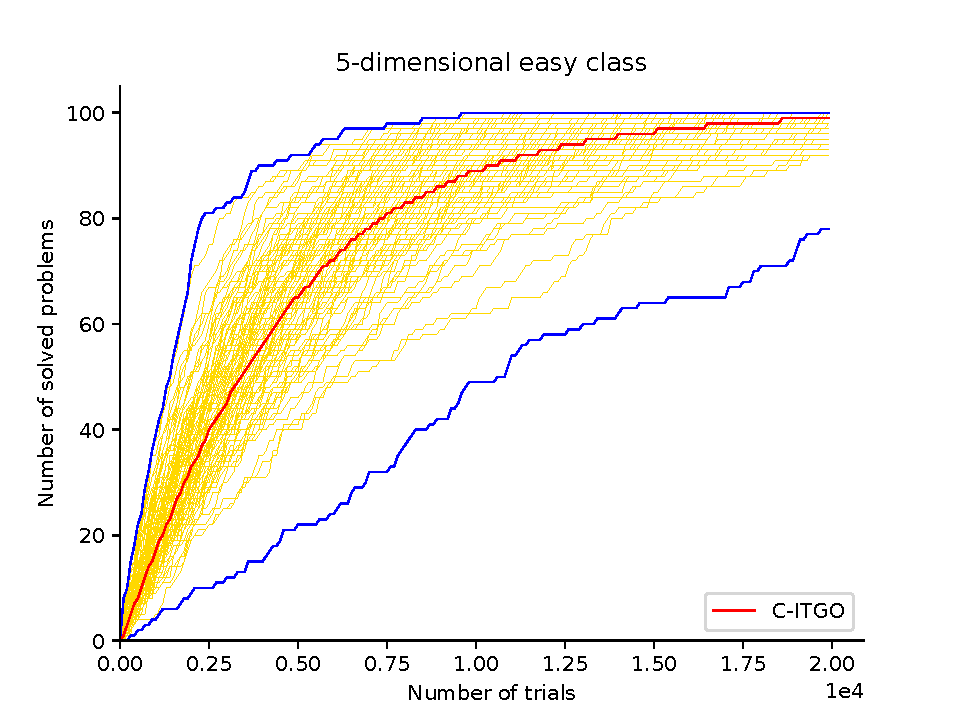
\includegraphics[width=1.1\linewidth]{img/GKLS/mult_5E}
      \caption{}
      \label{fig:OpZone_a}
    \end{subfigure}%
    \begin{subfigure}{.5\textwidth}
      \centering
      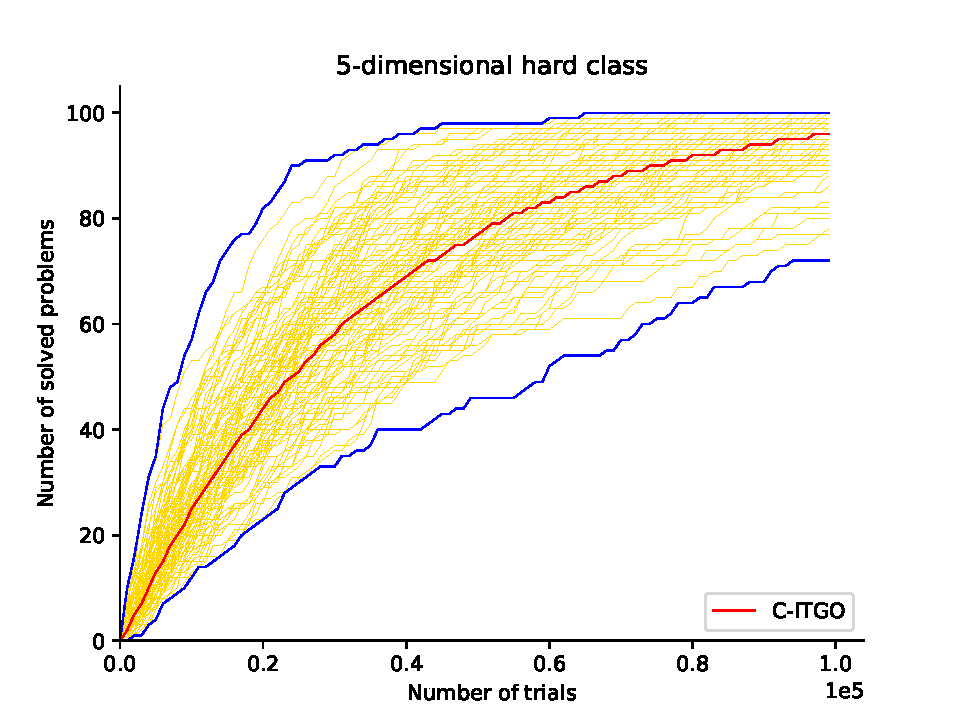
\includegraphics[width=1.1\linewidth]{img/GKLS/mult_5H}
      \caption{}
      \label{fig:OpZone_b}
    \end{subfigure}
    \caption{The operational zones built using the 10,000 runs performed by the C-ITGO algorithm for the five dimensional easy (a) and hard (b) cases. The lower and upper bounds are in blue, while the mean is in red.}\label{fig:OpZone}
\end{figure}


\begin{figure}[h]
    \centering
    \begin{subfigure}{.5\textwidth}
      \centering
      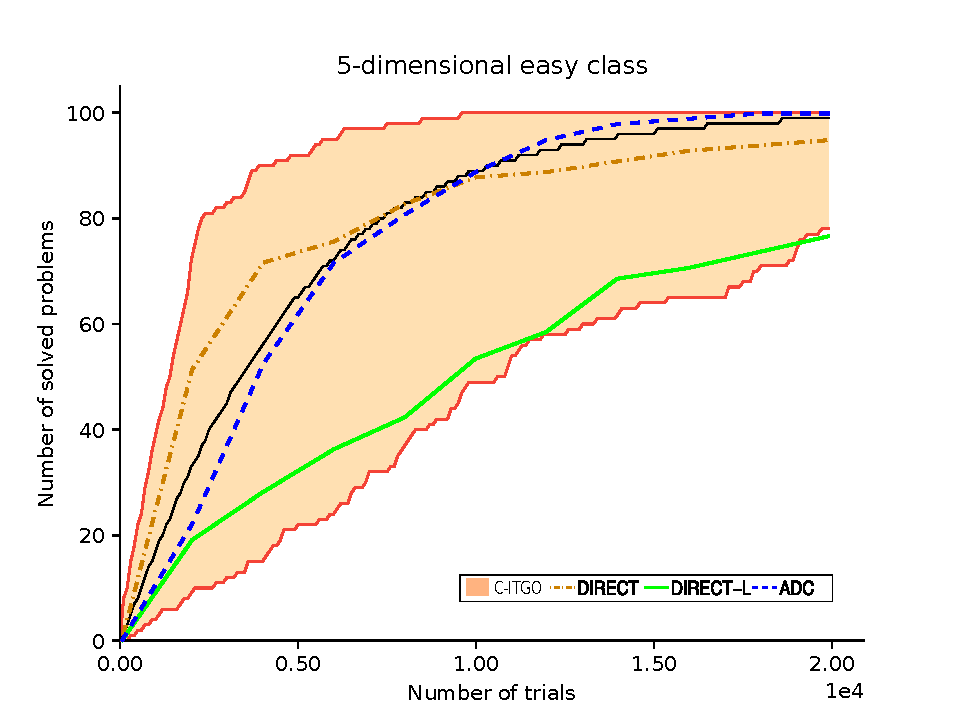
\includegraphics[width=1.1\linewidth]{img/GKLS/fill_5E_edit}
      \caption{}
      \label{fig:OpCarac_a}
    \end{subfigure}%
    \begin{subfigure}{.5\textwidth}
      \centering
      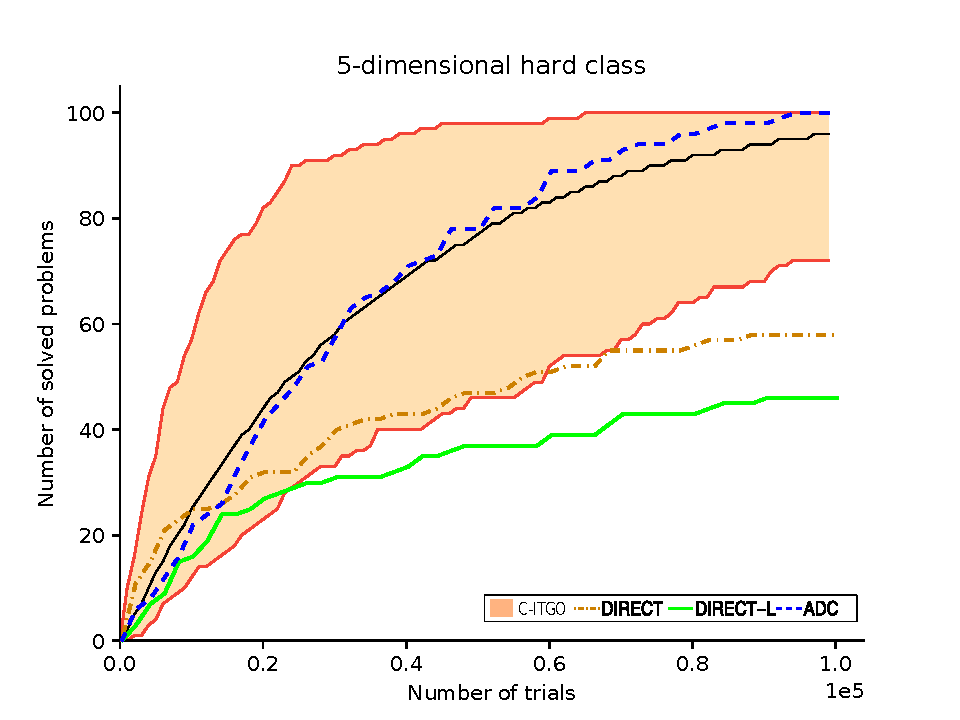
\includegraphics[width=1.1\linewidth]{img/GKLS/fill_5H_edit}
      \caption{}
      \label{fig:OpCarac_b}
    \end{subfigure}
    \caption{Operational zones built on the two 5-dimensional classes for the C-ITGO algorithm, and operational characteristics of the DIRECT, DIRECT-L and ADC methods.}\label{fig:OpCarac}
\end{figure}


However, the DIRECT-KS presents the best statistics in all the cases considered. Thus, we decided to execute a nonparametric statistical test, the Wilcoxon test \citep{Friedman} (which is very useful to compare the performance of two algorithms when applied to a common set of problems), to check if there is any statistically significant difference of performance between C-ITGO and the DIRECT-KS method.

Table \ref{tab:Wilcoxon2} shows the results generated using the \textit{wilcoxon.test} command of the R software, considering DIRECT-KS as reference/control against the other methods. 

\begin{table*}[h]
    \tiny
    \begin{center}
    
    \begin{tabular}{ P{1.0cm} P{1.0cm} P{1.2cm} P{1.0cm} P{1.0cm} P{1.0cm} }
                     &         &          &          &          &        \\[2em]
                     &  DIRECT & DIRECT-L &    ADC   &    SGEO-QN   & C-ITGO \\[1em]
    \cline{2-6}
    \rule{0pt}{3ex}
    \textbf{p-value} & 0.0416 & 0.0781 & 0.2154 & 0.0037 & 0.2818 \\


    \end{tabular}
    \end{center}
    \vspace*{-4mm}
    \captionsetup{justification=centering}
    \caption{Wilcoxon signed rank test comparing ADC against the other methods used to solve the GKLS class of problems. \\[2em]}
    \label{tab:Wilcoxon2}
\end{table*}

The ADC method shows an improvement over DIRECT and SGEO-QN with a level of significance of $\alpha$ = 0.05, and over DIRECT-L with a level of significance of $\alpha$ = 0.1. When compared to ADC and C-ITGO, the probability of presenting any significant statistical difference is bellow 80\%, what is indicated by a p-value greater than 0.2. 

When considering the eight different cases of the GKLS function generator, we can conclude that there is not any significant statistical difference between the C-ITGO and the ADC methods, showing that the performance of C-ITGO is equivalent to the DIRECT-KS over the GKLS generated problems considered in this work.

We would like to explore further the effectiveness of C-ITGO for the unconstrained case in a future work, possibly improving the current results.